\documentclass[11pt]{preprint}

\setlength{\topmargin}{0mm} \setlength{\oddsidemargin}{0mm}
\setlength{\textwidth}{160mm} \setlength{\textheight}{215mm}

\usepackage{amssymb,amsmath,amscd,amsthm}
\usepackage{graphics}
\usepackage{tikz}

\def\enumb{\begin{enumerate}}
\def\enume{\end{enumerate}}
\def\itemb{\begin{itemize}}
\def\iteme{\end{itemize}}
\def\integers{\mathbb{Z}}

\def\multiset#1#2{\ensuremath{\left(\kern-.3em\left(\genfrac{}{}{0pt}{}{#1}{#2}\right)\kern-.3em\right)}}



\newtheorem{proposition}{Proposition}
\newtheorem{theorem}{Theorem}

\title{Discrete Mathematics, 2016 Fall- Worksheet 11}
\author{Instructor: Zsolt Pajor-Gyulai, CIMS}
\date{October 19, 2016}



\begin{document}

\maketitle

In all of the above problems explain your answer in full English sentences.

\enumb
\item Show algebraically that
\[
\frac{(2k+1)(k+1)k}{6}+(k+1)^2=\frac{[2(k+1)+1][(k+1)+1][k+1]}{6}.
\]


\item Let $n$ be a positive integer. Prove the following equations and inequalities by induction.
\enumb
\item $1+4+7+\dots+(3n-2)=\frac{n(3n-1)}{2}$.


\item $9+9\times 10+9\times 100+\dots+9\times 10^{n-1}=10^{n}-1$.
\item $1\cdot 1!+2\cdot 2!+\dots+n\cdot n!=(n+1)!-1$.
\item $2^n\leq 2^{n+1}-2^{n-1}-1$.
\item $(1-\frac{1}{2})(1-\frac{1}{4})\cdot(1-\frac{1}{2^n})\geq\frac{1}{4}+\frac{1}{2^{n+1}}$.
\enume

\item Suppose that a grid has $a+1$ vertical lines and $b+1$ horizontal lines. Prove by strong  induction that there are $\binom{a+b}{a}$ lattice paths from the lower left to the upper right corner.


\begin{center}
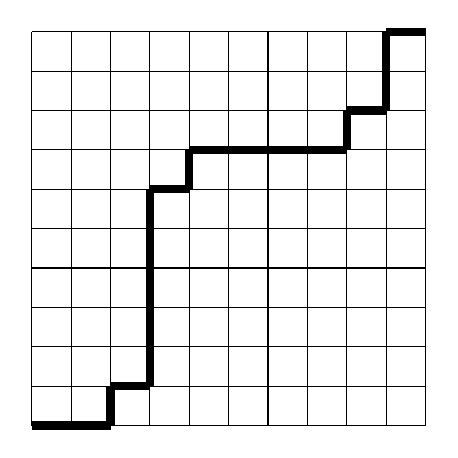
\begin{tikzpicture}[scale=0.5]
\foreach \i in {0,1,2,3,4,5,6,7,8,9,10}
	{
		\draw (\i,0) -- (\i,10);
	}
	
\foreach \i in {0,1,2,3,4,5,6,7,8,9,10}
	{
		\draw (0,\i) -- (10,\i);
	}
	
\draw[line width=3pt] (0,0) -- (2,0);
\draw[line width=3pt] (2,0) -- (2,1);
\draw[line width=3pt] (2,1) -- (3,1);
\draw[line width=3pt] (3,1) -- (3,6);
\draw[line width=3pt] (3,6) -- (4,6);
\draw[line width=3pt] (4,6) -- (4,7);
\draw[line width=3pt] (4,7) -- (8,7);
\draw[line width=3pt] (8,7) -- (8,8);
\draw[line width=3pt] (8,8) -- (9,8);
\draw[line width=3pt] (9,8) -- (9,10);
\draw[line width=3pt] (9,10) -- (10,10);

\end{tikzpicture}

Figure 2: Grid with $a=b=9$.
\end{center}
\item A flagpole is $n$ feet tall. On this pole, we display flags of the following types: red flags that are $1$ foot tall, blue flags that are $2$ feet tall, and green flags that are $2$ feet tall. The sum of the heights of the flags is exactly $n$ feet. Prove by induction that there are $\frac{2}{3}2^n+\frac{1}{3}(-1)^n$ ways to display the flags.

\item BONUS PROBLEM: Consider the following computer program.
\begin{verbatim}
function findMax(array, first, last){
  if (first==last) return array[first];
  mid = first+ (last-first)/2;
  a = findMax(array,first,mid); 
  b = findMax(array,mid+1,last);
  if (a<b) return b;
  return a;
}
\end{verbatim}
Here \verb array ~is an array of integers. All other variables are integers. We assume that \verb first ~and \verb last ~are between $1$ and the number of elements in \verb array ~and that \verb first $\leq$ \verb last . Note that if \verb last-first ~is odd, then (\verb last-first )/2 is rounded down to the nearest integer.

The purpose of this program is to find the largest value in the array between two indices; that is, it should return the largest value of
\begin{verbatim}
 array[first],array[first+1],...,array[last].
 \end{verbatim}
 Prove that this program fulfills this task.
\enume
\end{document}